\documentclass[tikz,border=10pt]{standalone}
\begin{document}
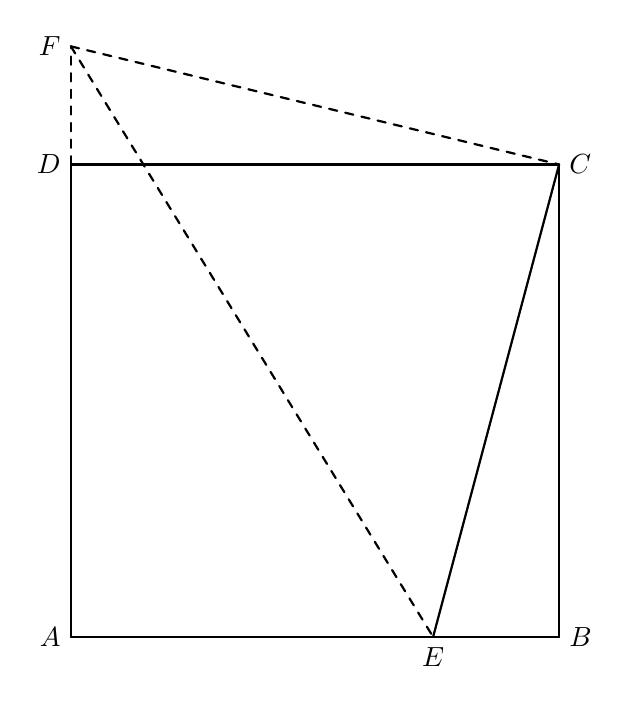
\begin{tikzpicture}[line cap=round,line join=round,thick]

\coordinate (A) at (0,0);
\coordinate (B) at (6.2,0);
\coordinate (C) at (6.2,6.0);
\coordinate (D) at (0,6.0);
\coordinate (E) at (4.6,0);
\coordinate (F) at (0,7.5);

\draw (A) -- (D) -- (C) -- (B);
\draw (A) -- (B);
\draw (E) -- (C);

\draw[dashed] (D) -- (F);
\draw[dashed] (F) -- (C);
\draw[dashed] (F) -- (E);

\node[left] at (A) {$A$};
\node[right] at (B) {$B$};
\node[right] at (C) {$C$};
\node[left] at (D) {$D$};
\node[below] at (E) {$E$};
\node[left] at (F) {$F$};

\end{tikzpicture}
\end{document}
